%%
%% Author: Maciej
%% 18.11.2018
%%

% Preamble
\documentclass[11pt]{article}

% Packages
\usepackage{amsmath}
\usepackage{pythontex}
\usepackage{graphicx}
\usepackage{caption}
\usepackage{float}
\restylefloat{table}

% Document
\begin{document}
\begin{pythontexcustomcode}{py}
import pickle
def architecture_table_5(network_architecture):
    print(r"\begin{table}[H]")
    print(r"\begin{tabular}{c|c|c|c|c|c}")
    print(r"\centering")
    table_row = ' '
    for layer in network_architecture.values():
        table_row += ' & ' + layer['activation_function']
    print(r"{0} \\".format(table_row))
    table_row = '\LARGE 748 '
    for layer in network_architecture.values():
        table_row += r"& \LARGE {0}".format(layer['size'])
    print(r"{0} \\".format(table_row))
    table_row = ' '
    for layer in network_architecture.values():
        table_row += '& ' + str(layer['dropout'])
    print(r"{0}".format(table_row))
    print(r"\end{tabular}")
    print(r"\end{table}")
    print(r"\captionof{table}{Network architecture}")
\end{pythontexcustomcode}
\begin{pycode}
with open('network_architecture.pickle', 'rb') as f:
    network_architecture = pickle.load(f)
if len(network_architecture.keys()) == 5:
    architecture_table_5(network_architecture)
\end{pycode}
    \begin{figure}[h!]
        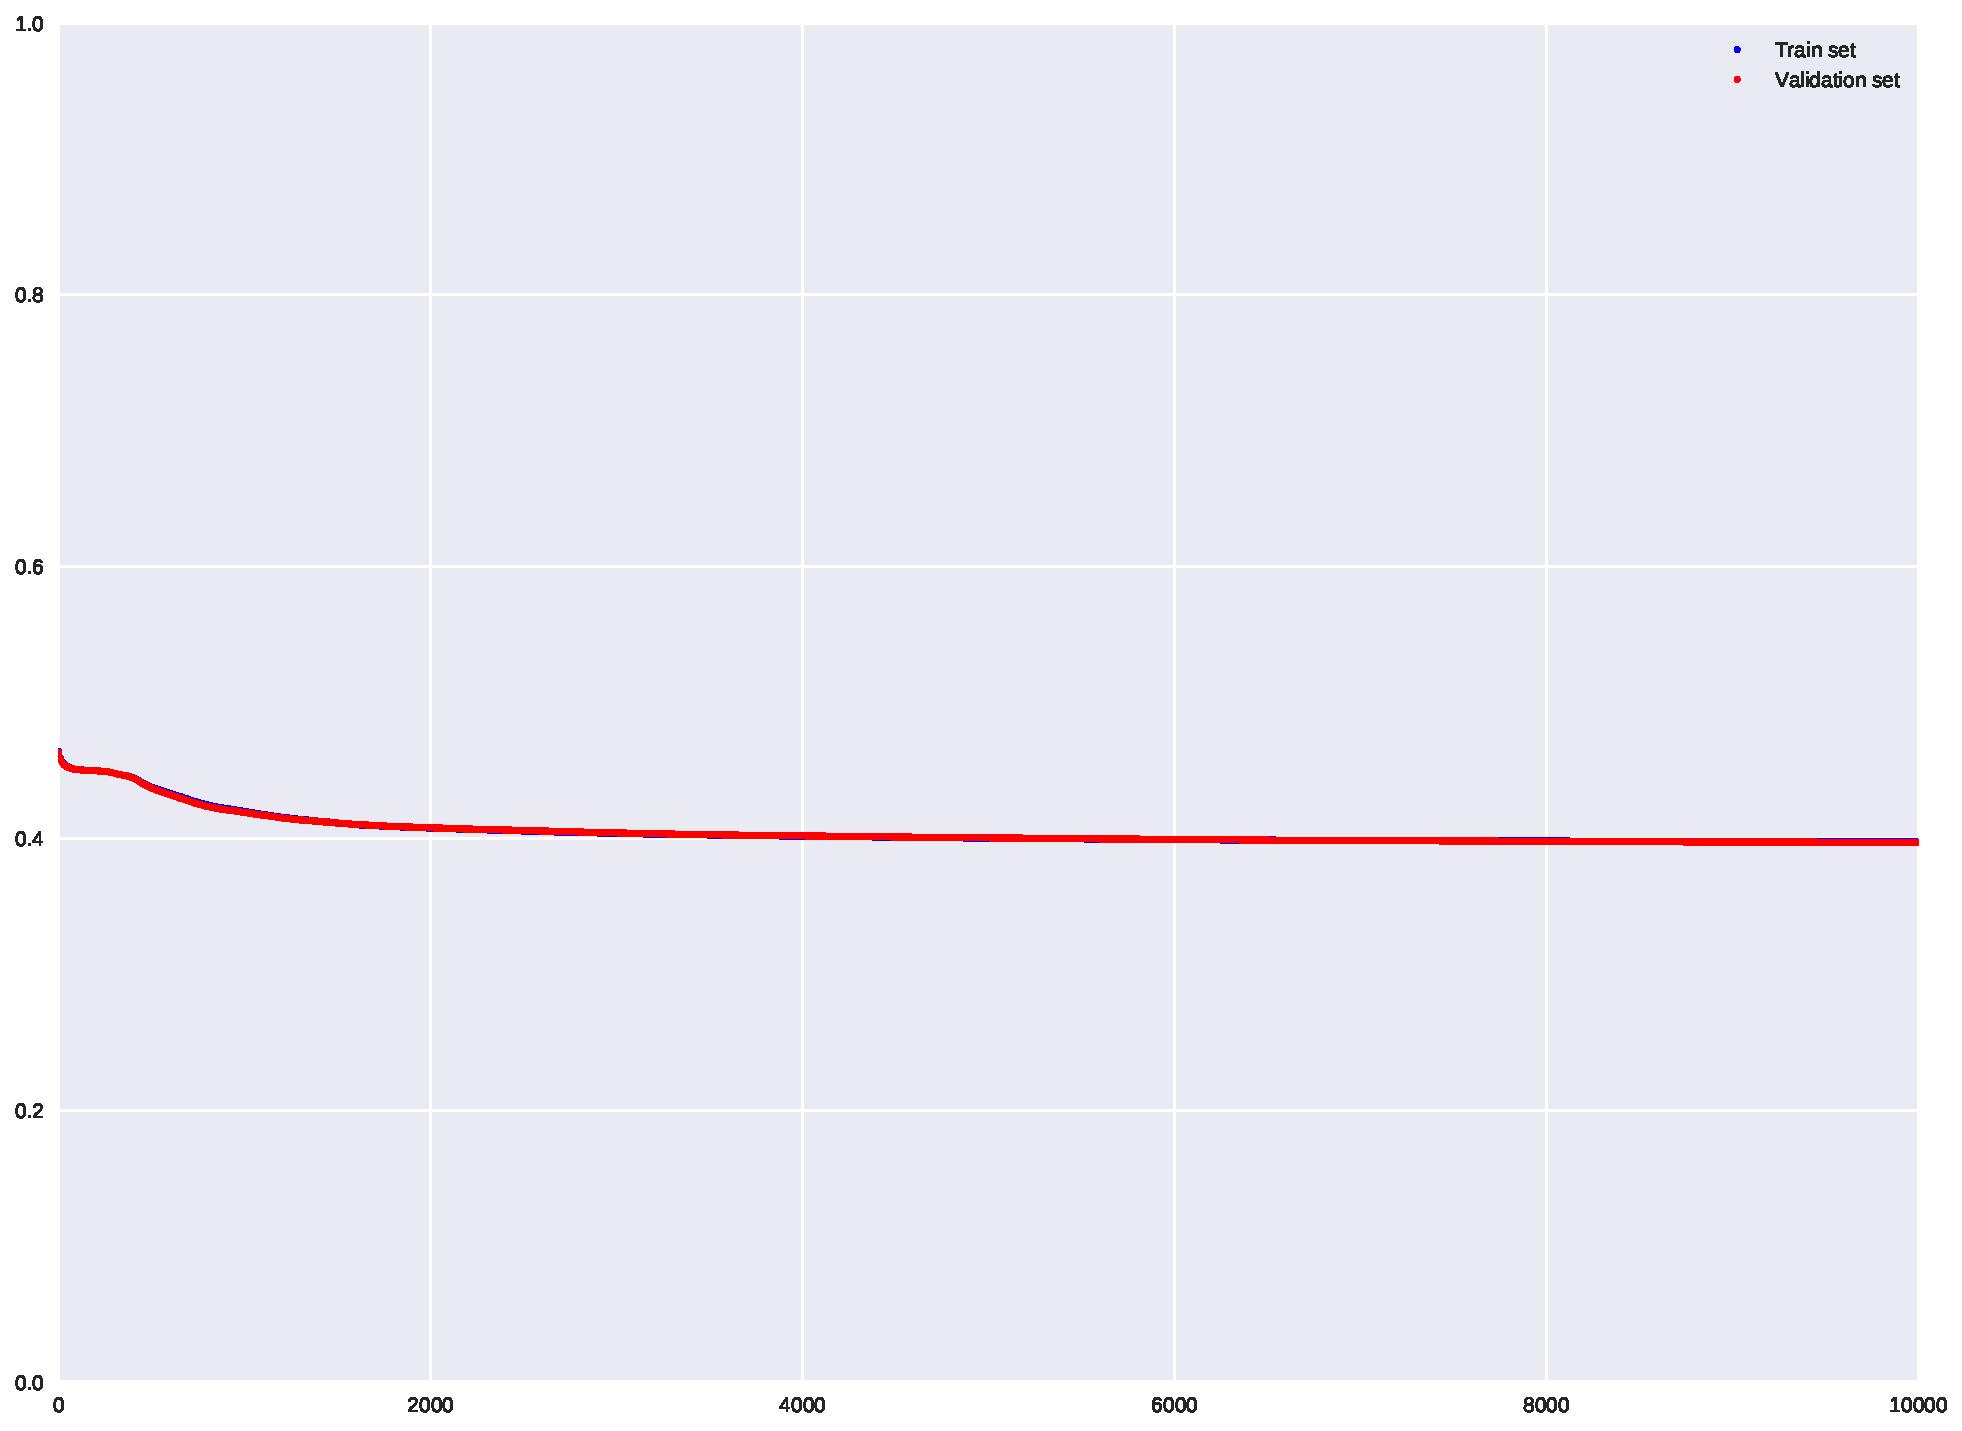
\includegraphics[width=\textwidth]{learning_curves.pdf}
        \caption{Euclidean distance errors for consecutive learning epochs}
    \end{figure}
\end{document}